\documentclass{article}
\usepackage[margin=1in]{geometry}
\usepackage{amsmath,amssymb,booktabs,multirow,graphicx}
\usepackage{xcolor}
\usepackage[colorlinks=true,citecolor=blue]{hyperref}

\newcommand{\R}{\mathbb{R}}
\newcommand{\gN}{\mathcal{N}}
\newcommand{\ess}{\text{ESS}}

\begin{document}

\section{Cosmology: DES Y1 \texorpdfstring{$3\times 2$pt}{3x2pt}}\label{sec:desY1}

\emph{Scope note.} This is the PICKLES-focused note: the headline
comparison is Metropolized PICKLES against NUTS (\texttt{NumPyro}) and
\texttt{emcee}. The broader benchmark of all additional ensemble and
gradient samplers we ran on the same posterior (peaches, peams, peanuts,
chess, MALT, ALDI, \texttt{langevin\_walk}) is in the companion note
\texttt{des\_section\_v1\_many\_samplers.tex}. All results are
regenerable; see \texttt{results/des\_y1/MANIFEST.md} for the
directory-to-table map.

We close the experiments with the Dark Energy Survey Year~1 (DES~Y1)
$3\times 2$pt cosmological inference \cite{abbott2018dark,krause2017dark},
implemented through the \texttt{JAX-COSMO} forward model
\cite{campagne2023jax}. The posterior is $D=21$ dimensional, with the
standard cosmology reparametrization (logit transform on the 13 Uniform
priors and non-centered location-scale on the 8 Gaussian priors).
Empirically the posterior has condition number $\kappa(\Sigma)\!\approx\!300$,
with six parameter pairs at $|\rho|>0.9$ — all between $\sigma_8$ and
the five galaxy bias parameters $b_{1\!:\!5}$ — and eight prior-dominated
nuisance directions. Figure~\ref{fig:desCorner} illustrates the posterior
geometry; full likelihood and prior specification follow Campagne et al.
\cite{campagne2023jax}.

\begin{figure}[t]
\centering
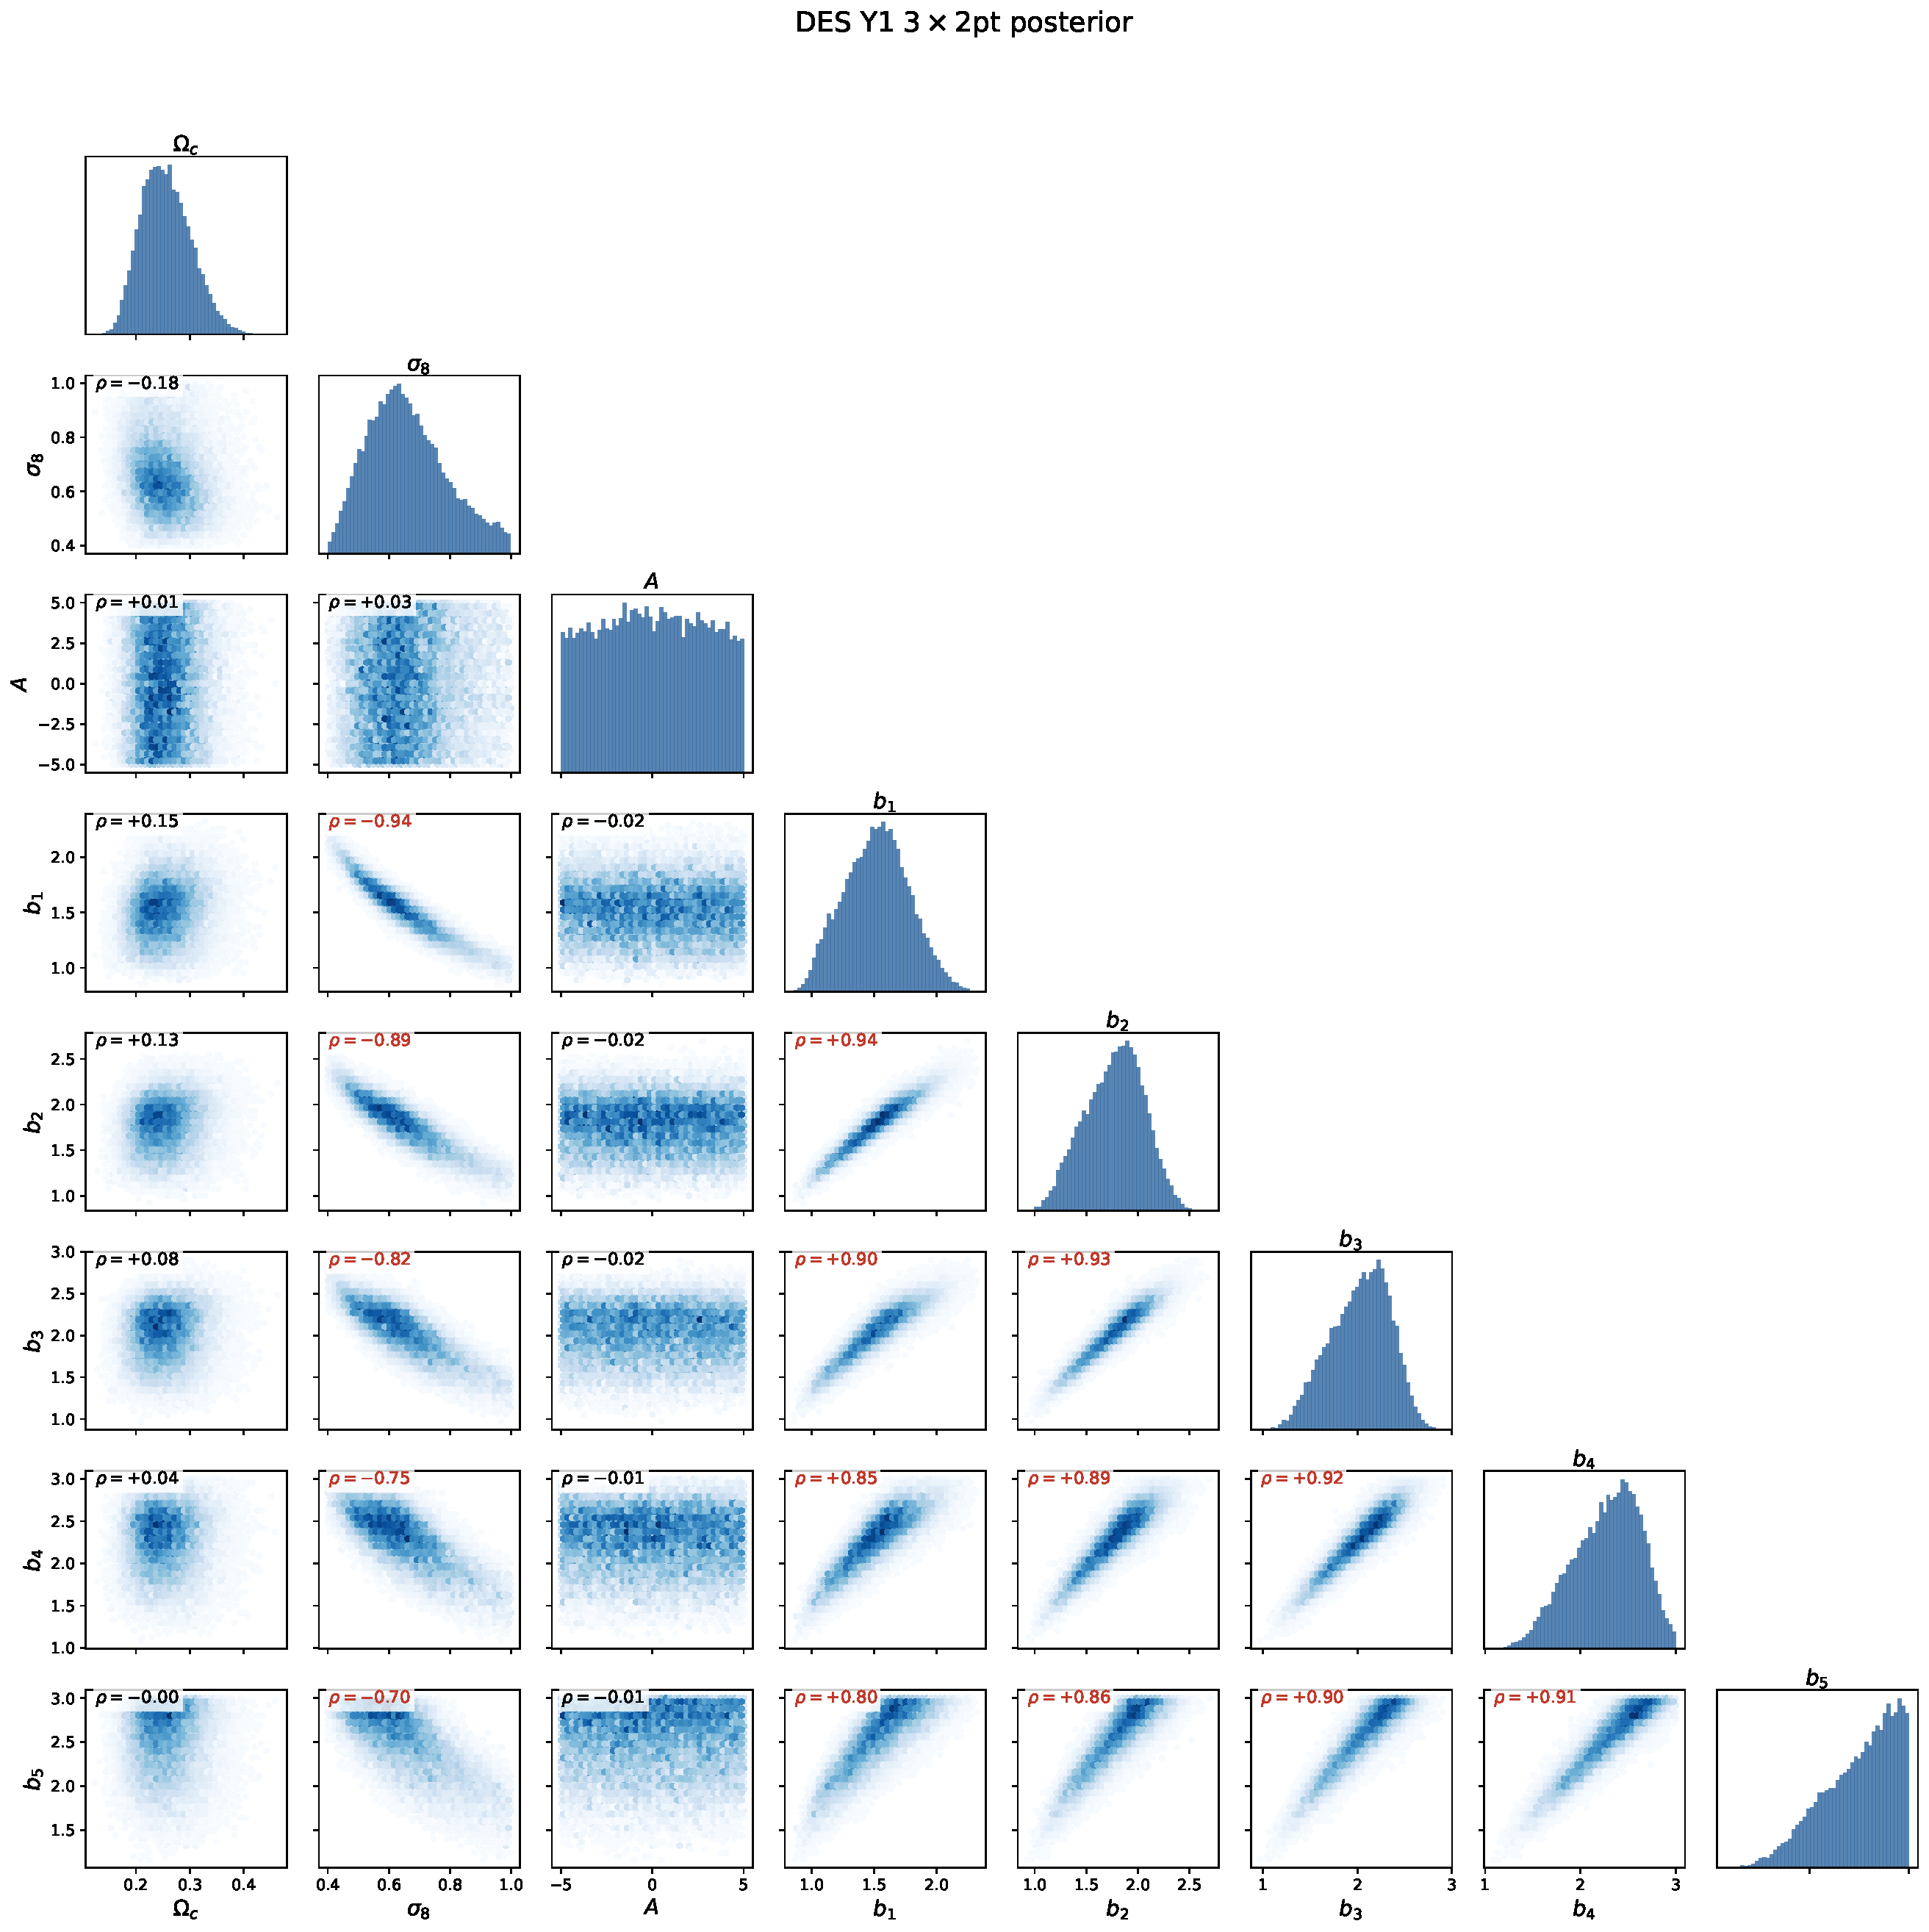
\includegraphics[width=0.95\linewidth]{figs/des_y1_corner_optB.pdf}
\caption{DES~Y1 $3\times 2$pt posterior, eight \emph{sampled}
marginals of $D=21$.  The two control panels (rows $\Omega_c$, $A$)
show near-isotropic ellipses with $|\rho| \le 0.2$, while every
panel involving $\sigma_8$ and the five galaxy biases $b_{1:5}$ shows
a narrow ridge ($|\rho|$ from $0.70$ to $0.94$, red text).  The
slow-mixing $6$-dim subspace consists entirely of $\sigma_8 + b_{1:5}$
(\S\ref{ssec:desMain}); the remaining $13$ dimensions
($\Omega_b$, $h$, $n_s$, $w_0$, $\eta$, $m_{1:4}$, $\Delta z_{1:4}$)
mix to the trivial upper bound and are not shown.}
\label{fig:desCorner}
\end{figure}

\begin{figure}[t]
\centering
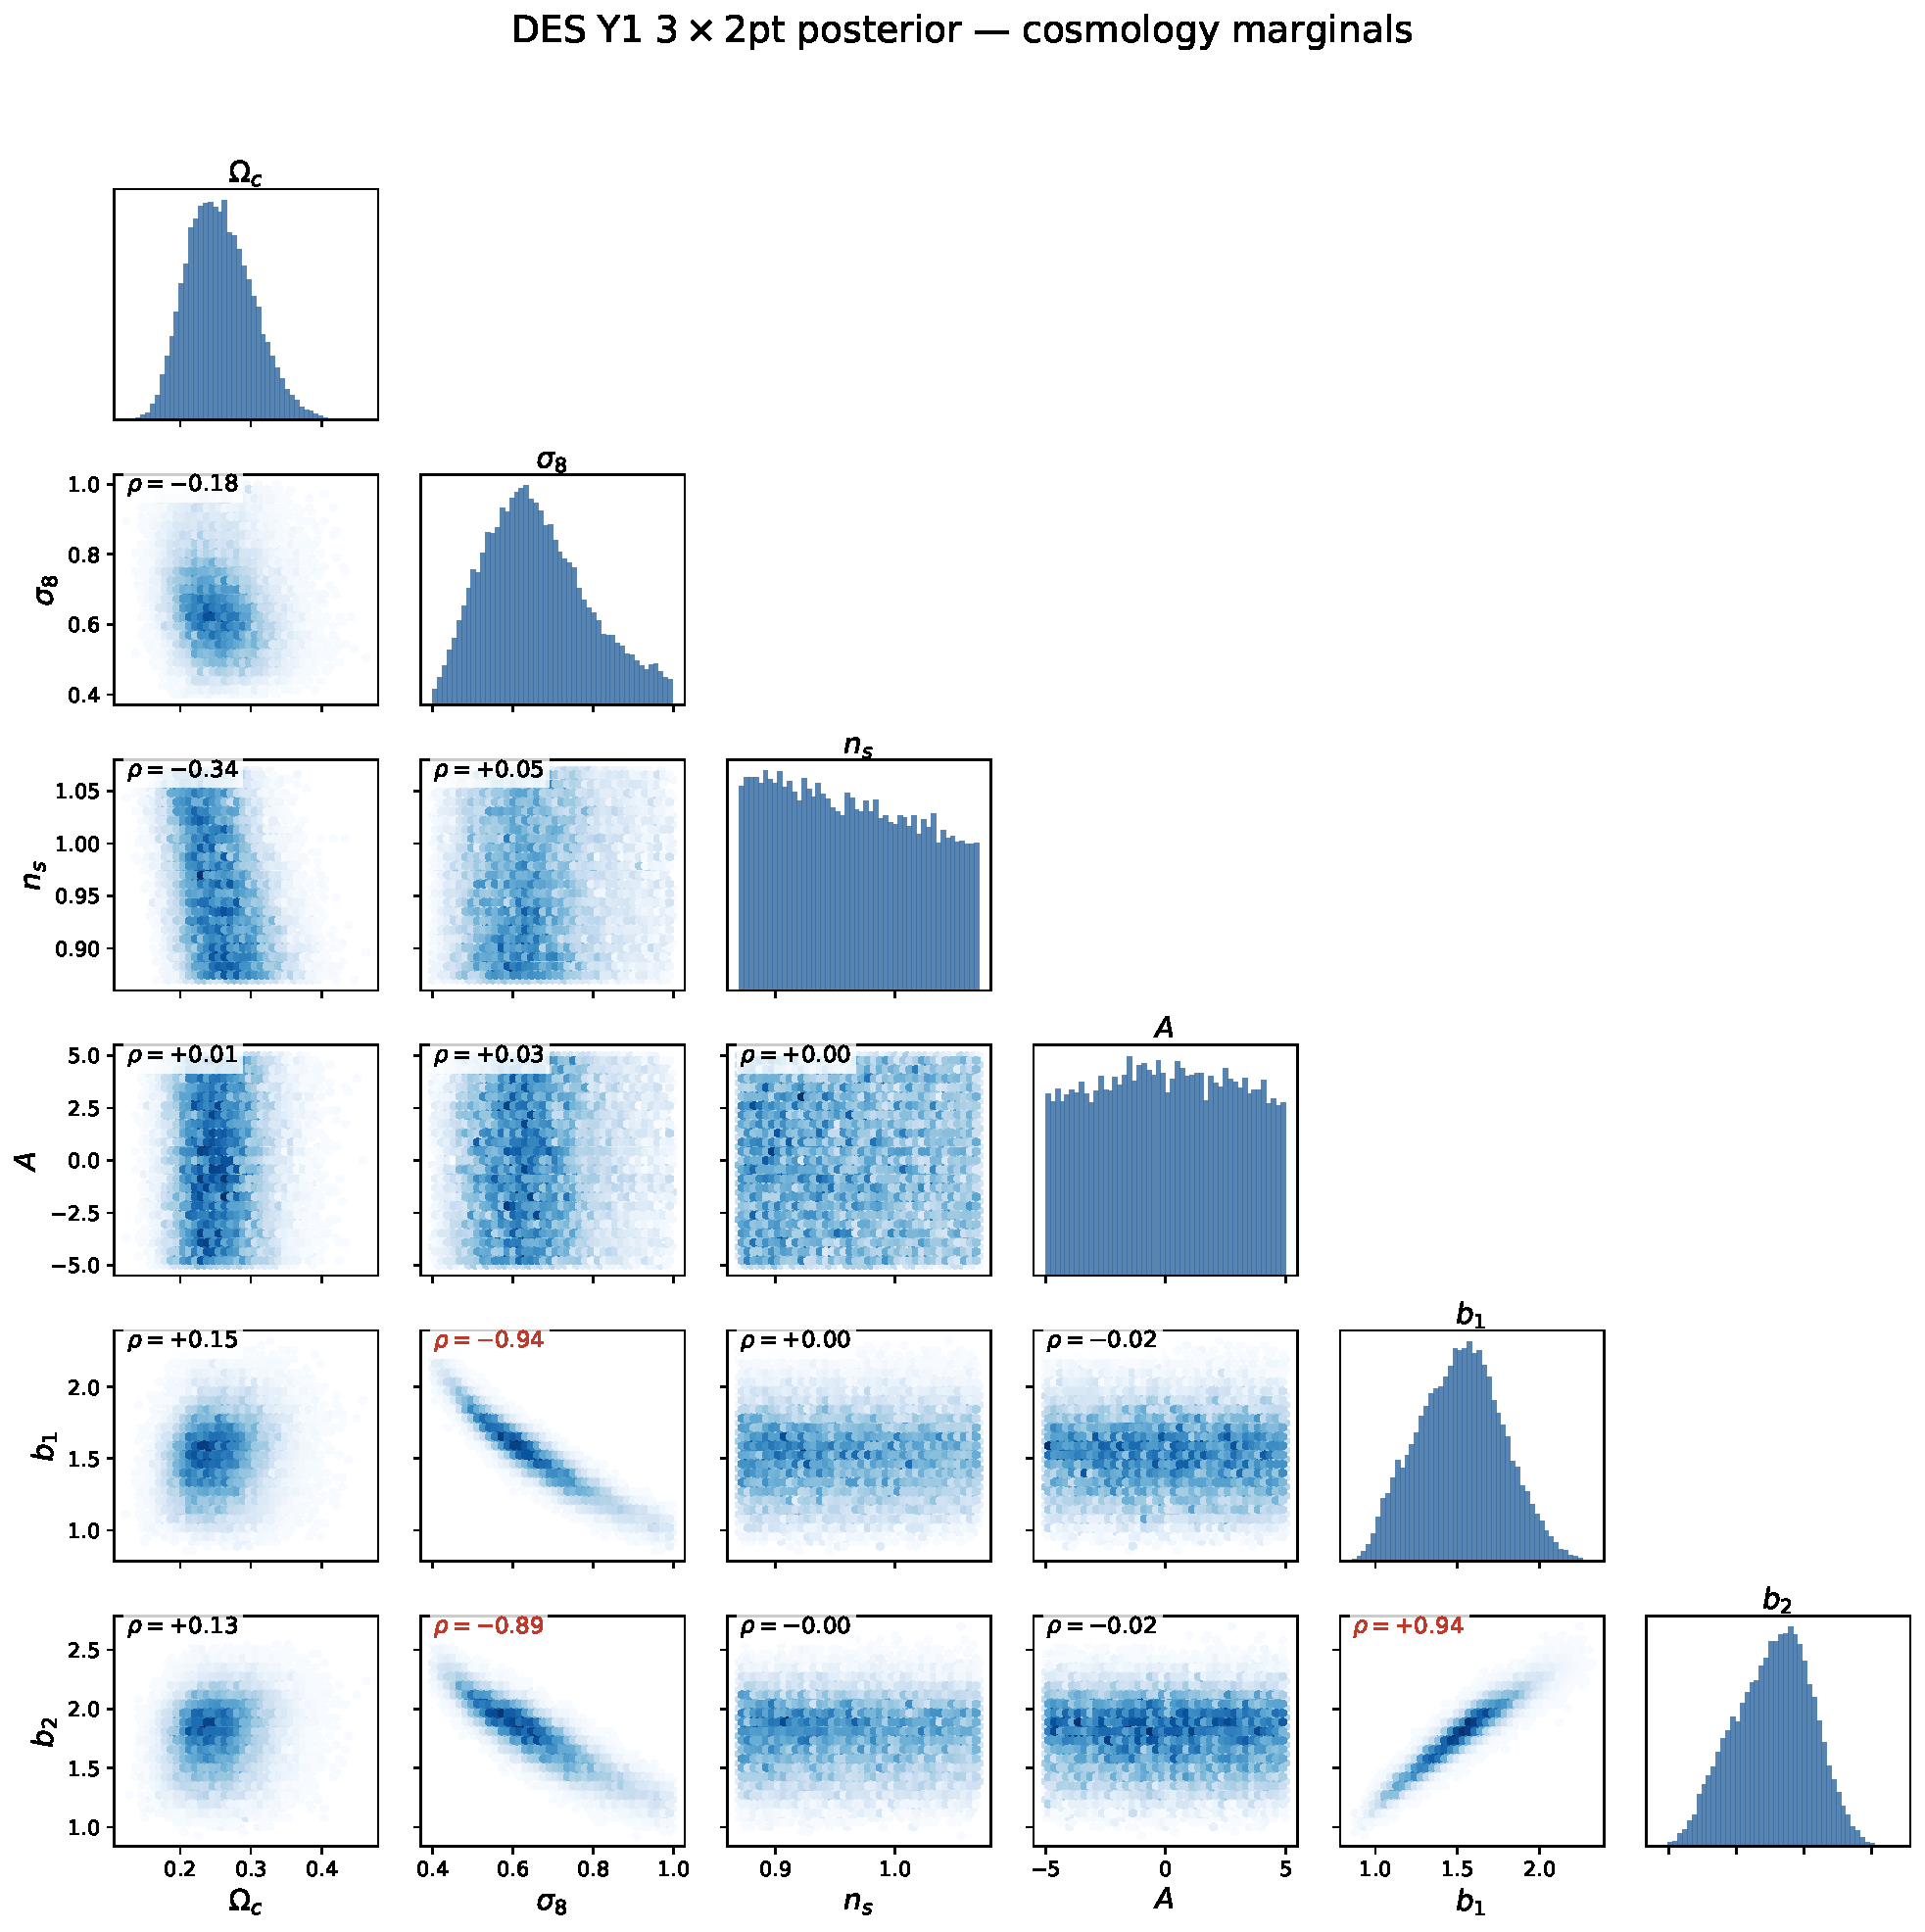
\includegraphics[width=0.49\linewidth]{figs/des_y1_corner_optC1.pdf}
\hfill
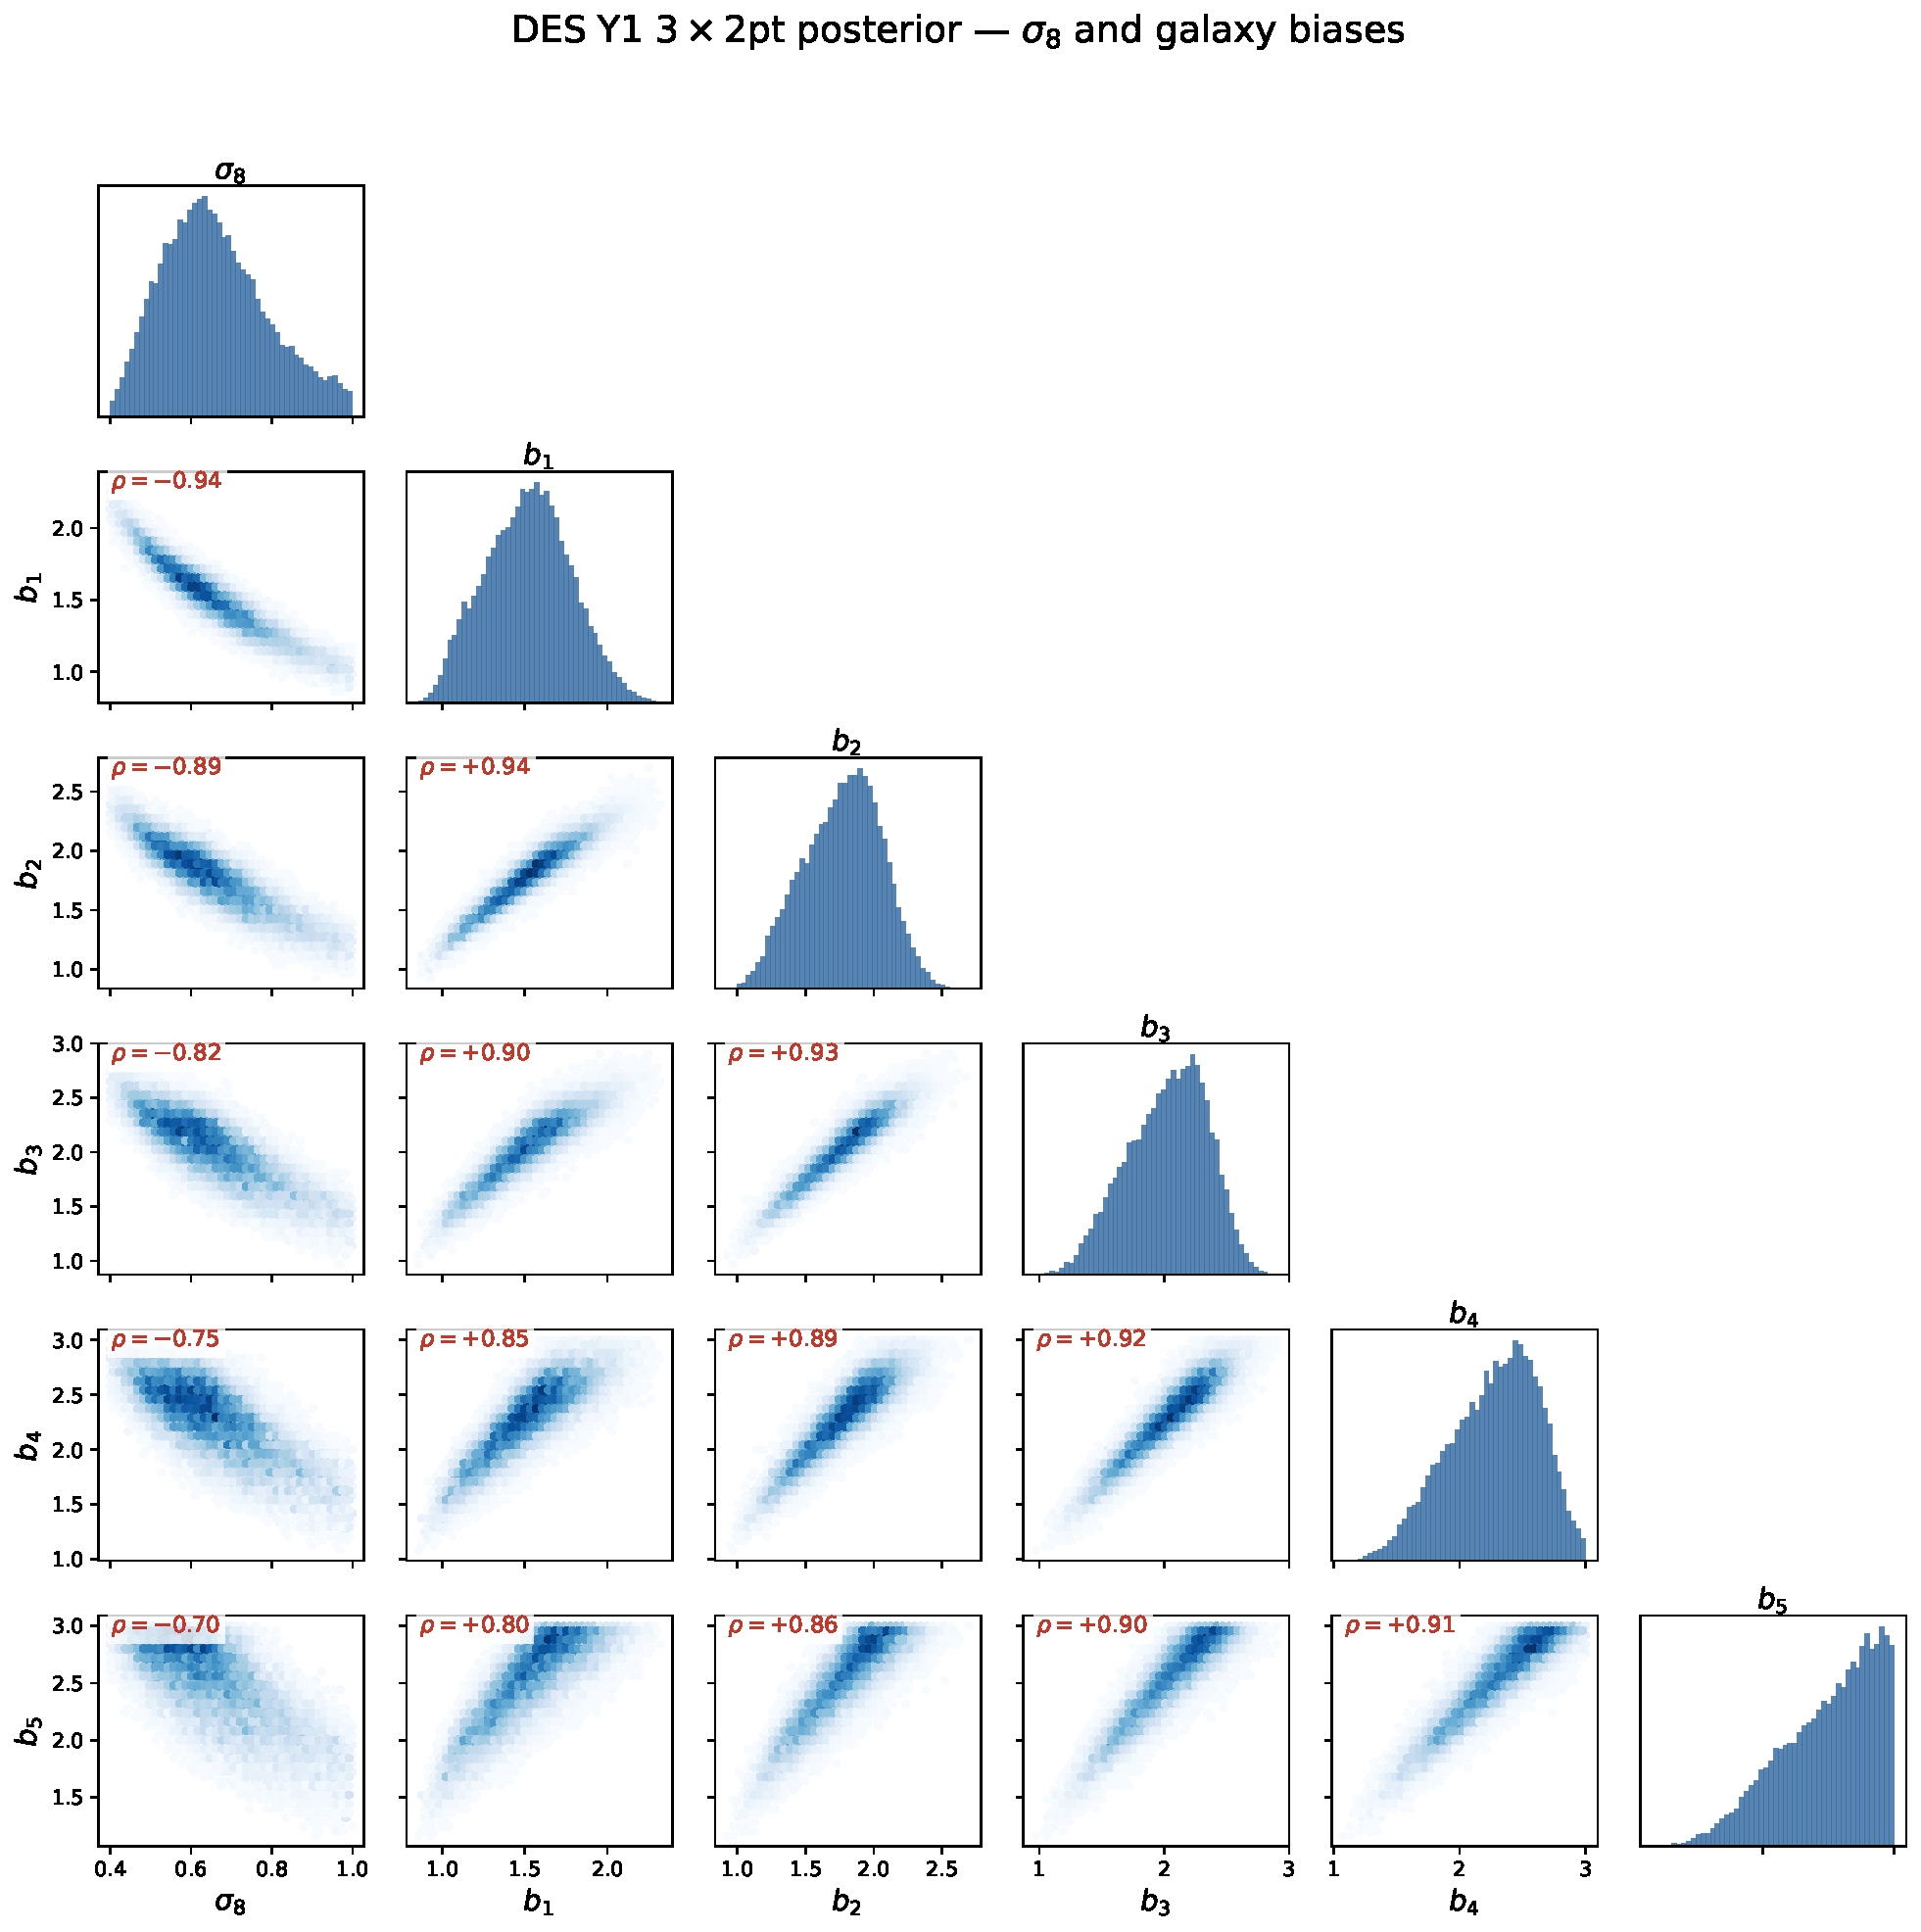
\includegraphics[width=0.49\linewidth]{figs/des_y1_corner_optC2.pdf}
\caption{Alternative six-dimensional views of the posterior.  Left:
the conventional cosmology-style corner ($\Omega_c$, $\sigma_8$,
$n_s$, $A$, $b_1$, $b_2$) showing three ridges
($\sigma_8\!\leftrightarrow\!b_1$,
$\sigma_8\!\leftrightarrow\!b_2$, $b_1\!\leftrightarrow\!b_2$,
each at $|\rho| \approx 0.94$).  Right: the slow subspace
($\sigma_8$ + the five galaxy biases $b_{1:5}$), in which every
off-diagonal panel is a narrow ridge ($|\rho|$ from $0.70$ to $0.94$);
this is the $6$-dim subspace responsible for the ESS bottleneck in
Table~\ref{tab:desPerDimEss}.}
\label{fig:desCornerSupp}
\end{figure}

In cosmological inference Metropolis-adjusted samplers are the
standard choice — they guarantee an unbiased target distribution at
any step size and avoid numerical divergence. We therefore consider
only Metropolized samplers in the main text and report unadjusted
variants in Appendix~\ref{app:desUnadjusted}. We compare
\textbf{Metropolized PICKLES} (the BAB-O variant with OBABO Metropolis
correction; Algorithm~\ref{alg:PicklesBABO} in the main text) at the
recommended tuning ($\gamma\!=\!0.5$, $L_{\max}\!=\!20$) against two
reference samplers widely used in astrophysical inference:
\textbf{emcee} \cite{foreman2013emcee} (the affine-invariant
gradient-free stretch move \cite{goodman2010ensemble}, the de-facto
default in the cosmology literature), and \textbf{NUTS-dense}
(\texttt{NumPyro} \cite{phan2019composable}, with a full $21\!\times\!21$
dual-averaging mass matrix; Campagne~et~al.\ \cite{campagne2023jax}
identify a block-dense variant of NUTS as the best-performing sampler
on this likelihood).

\textbf{Configuration.} PICKLES uses $N_{\text{ch}}\!=\!64$ ensemble
walkers parallelized via \texttt{jax.vmap} on a single NVIDIA H100
GPU; \texttt{emcee} uses the same ensemble configuration. NUTS uses
$N_{\text{ch}}\!=\!4$ chains run \emph{sequentially}
(\texttt{chain\_method="sequential"}, the \texttt{numpyro} default;
the four chains run one after another, so the per-chain wall is
roughly the total wall divided by four), with \texttt{init\_to\_median}
initialization, max-tree-depth $7$, and target acceptance $0.8$.
Walkers are initialized in a Gaussian ball of width $0.5$ (in
unconstrained $z$-space) around the fiducial cosmology. Each chain
runs $500$ warmup iterations and $5{,}000$ production iterations.
We report ESS\,/\,grad as the production-only count (warmup gradients
are excluded). \emph{Divergences} (a NUTS diagnostic): the count of
production iterations on which the leapfrog energy error exceeded the
default \texttt{numpyro} threshold ($1000\,k_B T$ in the Hamiltonian
analogy, configurable via \texttt{max\_delta\_energy}); a non-zero
divergence count indicates the integrator is unstable along part of
the typical set, and is the standard signal that the dual-averaged
mass matrix or step size is mistuned.

\paragraph{Note on cross-table variation.}
Each configuration choice (stretch pre-warmup $w_s$, gradient-sampler
warmup $w$, initialization, production length $N$, number of seeds)
gives slightly different ESS/grad numbers.  Table captions specify each
table's exact configuration; for clarity we collect the recommended
PICKLES~$\gamma{=}0.5$, $L_{\max}{=}20$ headline numbers and the
NUTS-dense reference here:
\begin{itemize}\setlength\itemsep{1pt}
\item Main comparison (Table~\ref{tab:desMainN1k}): $N{=}1000$,
$w_s{=}0$, $w{=}500$, fid-ball init, $3$-seed median ---
PICKLES $\gamma=0.5$: $5.56\!\times\!10^{-3}$; NUTS-dense:
$4.69\!\times\!10^{-3}$.
\item Long-production reference (Table~\ref{tab:desMainN5k}):
$N{=}5000$, same init/$w_s$/$w$, single seed ---
PICKLES $\gamma=0.5$: $4.09\!\times\!10^{-3}$; NUTS-dense:
$3.72\!\times\!10^{-3}$.  (Longer $N$ resolves more autocorrelation
tail, lowering both numbers $\sim\!25$\%.)
\item Per-parameter breakdown
(Table~\ref{tab:desPerDimEss}): same config as
Table~\ref{tab:desMainN1k} ($w_s{=}0$, fid-ball, $w{=}500$, $3$-seed
median, $N{=}1000$), with the only difference being that the per-dim
table reports uncapped $\hat\tau$ (allowing $\hat\tau < 1$ for the
antithetic-HMC NUTS chains, which can show ESS\,/\,grad above
$3\!\times\!10^{-2}$ in the fast subspace). Worst-dim values:
PICKLES $\gamma=0.5$ $\sigma_8$ ESS\,/\,grad $= 5.56\!\times\!10^{-3}$
(matches Table~\ref{tab:desMainN1k}); NUTS-dense $b_5$ ESS\,/\,grad
$= 5.90\!\times\!10^{-3}$.
\item Warmup robustness (Table~\ref{tab:desWarmupSweep}): grid of
$w \in \{50, 100, 150, 200\}$ and $w_s \in \{0, 50, 200\}$ ---
PICKLES~$\gamma=0.5$ recommended ($w_s{=}200$) is uniformly
$5\!\times\!10^{-3}$; the same sampler at $w_s{=}0$ has stochastic
ridge collapse independent of $w$ (\S\ref{ssec:desWarmupSweep},
Appendix~\ref{app:desPerSeed}), median values shuffle between
collapsed ($\sim\!5\!\times\!10^{-4}$) and clean
($\sim\!5\!\times\!10^{-3}$) depending on seed assignment.
\end{itemize}

In what follows, the \emph{headline} comparison is
Table~\ref{tab:desMainN1k}; other tables either drill into a specific
aspect (long $N$, per-dim breakdown, warmup robustness) or are deferred
to the appendix (per-seed details, unadjusted methods).

\subsection{PICKLES is competitive with emcee and NUTS-dense}\label{ssec:desMain}

Table~\ref{tab:desMainN1k} reports ESS per gradient evaluation
(production-only) and wall-clock for each method, with three PICKLES
$L_{\max}$ choices reported alongside the default $\gamma=2$ tuning
and the NUTS / \texttt{emcee} reference samplers.

PICKLES at the recommended tuning ($\gamma=0.5$, $L_{\max}=20$)
achieves $\text{ESS}/\text{grad}\!=\!5.56\!\times\!10^{-3}$,
$1.18\!\times$ ahead of NUTS-dense, $1.38\!\times$ ahead of NUTS-block,
$2.45\!\times$ ahead of NUTS-diag, and $19\!\times$ ahead of
\texttt{emcee}. The kinetic-damping coefficient $\gamma$ is the
dominant tuning knob: switching from the default $\gamma=2$ to
$\gamma=0.5$ improves ESS\,/\,grad by $1.5\!\times$
(consistent with the linearized-Gaussian convergence-rate analysis of
\S\ref{ssec:antisymmetric1D}, which favors $\gamma=2$ for an
isotropic Gaussian but allows lower damping when the empirical
preconditioner already absorbs scale anisotropy). Increasing $L_{\max}$
from $20$ to $128$ produces $2.5\!\times$ more raw ESS but costs
$3\!\times$ more wall and reduces ESS\,/\,grad by $1.5\!\times$:
larger $L$ gives more exploration per sample but only sub-linearly
more independent samples per gradient. $L_{\max}=20$ is the per-grad
sweet spot.

PICKLES reports zero numerical divergences across all four configurations.
NUTS-dense reports $24$ divergences on $5{,}000$ samples in the
long-production reference (Table~\ref{tab:desMainN5k}); on
short-production-warmup combinations NUTS divergences can be much
larger (Table~\ref{tab:desWarmupSweep}).

\begin{table}[t]
\centering
\caption{DES Y1 $3\times 2$pt sampler comparison at the standard
production length, $N_{\text{prod}} = 1000$ samples per chain
(multi-seed median over $3$ seeds, FAIR-NO-WS init: walkers initialized
in a Gaussian ball of width $0.5$ in $z$-space around the fiducial
cosmology; no stretch pre-warmup). All runs use $500$ gradient-sampler
warmup iterations on a single NVIDIA H100 GPU. ESS denotes the
minimum effective sample size across the $21$ posterior dimensions;
ESS\,/\,eval is the production-only count of \emph{target evaluations}
— gradient evaluations for HMC, log-probability evaluations for
\texttt{emcee}. The mean trajectory length $\bar L$ is fixed for
PICKLES (set to $L_{\max}=20$) but adaptive for NUTS via the
no-U-turn criterion. NUTS-block has $\bar L \approx 63$ (vs $\bar
L \approx 33$ for NUTS-dense) because the block-diagonal mass-matrix
structure is mis-specified for this posterior: it does not capture
the $|\rho| \approx 0.94$ $\sigma_8$-bias cross-correlations
(Figure~\ref{fig:desCorner}), so the chain takes nearly twice as
many leapfrog steps per sample before satisfying the U-turn
termination condition.}
\label{tab:desMainN1k}
\small
\begin{tabular}{l rrrr rr}
\toprule
& $N_{\text{ch}}$ & wall (h) & $\bar L$ & acc.
& ESS & ESS\,/\,eval \\
\midrule
\multicolumn{7}{l}{\emph{Metropolized PICKLES (this work) — three values of the trajectory cap $L_{\max}$:}} \\
\textbf{PICKLES} ($\gamma=0.5$, $L_{\max}=20$, recommended)
   & 64 & 1.6 & 20.0 & 0.95
   & 7{,}113 & $\mathbf{5.56\!\times\!10^{-3}}$ \\
PICKLES ($\gamma=0.5$, $L_{\max}=50$)
   & 64 & 3.4 & 49.8 & 0.93
   & 14{,}695 & $4.61\!\times\!10^{-3}$ \\
PICKLES ($\gamma=0.5$, $L_{\max}=128$)
   & 64 & 4.8 & 93.4 & 0.92
   & 17{,}517 & $3.60\!\times\!10^{-3}$ \\
PICKLES (default $\gamma=2$, $L_{\max}=20$)
   & 64 & 1.6 & 20.0 & 0.94
   & 4{,}660 & $3.64\!\times\!10^{-3}$ \\
PICKLES (default $\gamma=2$, $L_{\max}=50$)
   & 64 & 3.4 & 49.8 & 0.92
   & 8{,}430 & $2.65\!\times\!10^{-3}$ \\
PICKLES (default $\gamma=2$, $L_{\max}=128$)
   & 64 & 5.3 & 78.3 & 0.90
   & 9{,}314 & $1.88\!\times\!10^{-3}$ \\
\midrule
\multicolumn{7}{l}{\emph{Reference samplers:}} \\
NUTS-dense (\texttt{numpyro})
   & 4 & 8.4 & 33 & 0.80
   &   787 & $4.69\!\times\!10^{-3}$ \\
NUTS-block (Campagne+ structure)
   & 4 & 11.3 & 63 & 0.80
   & 1{,}013 & $4.03\!\times\!10^{-3}$ \\
NUTS-diag
   & 4 & 12.5 & 83 & 0.80
   &   746 & $2.27\!\times\!10^{-3}$ \\
\texttt{emcee} / stretch (gradient-free)
   & 64 & 0.05 & --- & 0.27
   &     18 & $2.87\!\times\!10^{-4}$ \\
\bottomrule
\end{tabular}
\end{table}

A long-production-run reference is reported in
Table~\ref{tab:desMainN5k} at $N_{\text{prod}} = 5000$. Going to longer
production length reduces the autocorrelation-truncation bias of the
Sokal estimator at the cost of $5\times$ more wall time; the relative
ranking of the methods is preserved.

\begin{table}[t]
\centering
\caption{DES Y1 $3\times 2$pt long-production-run reference at
$N_{\text{prod}} = 5000$, single seed (parameters and hardware as in
Table~\ref{tab:desMainN1k}). \texttt{emcee} uses
$N_{\text{prod}} = 50{,}000$ since the gradient-free stretch move has
long autocorrelation tails. On HMC variants, the per-grad numbers are
$\sim\!1.5$--$3\times$ lower than at $N=1{,}000$ because the Sokal
estimator now sees the full autocorrelation tail; the asymptotic
ranking is preserved.}
\label{tab:desMainN5k}
\small
\begin{tabular}{l rrrrr rr}
\toprule
& $N_{\text{ch}}$ & wall (h) & $\bar L$ & acc. & div.
& ESS & ESS\,/\,eval \\
\midrule
\textbf{PICKLES} ($\gamma=0.5$, $L_{\max}=20$) & 64 & 5.0 & 20.0 & 0.94 & 0
   & 26{,}151 & $\mathbf{4.09\!\times\!10^{-3}}$ \\
PICKLES (default $\gamma=2$)
   & 64 & 4.8 & 20.0 & 0.99 & 0
   & 7{,}553 & $1.18\!\times\!10^{-3}$ \\
NUTS-dense (\texttt{numpyro}) & 4 & 10.2 & 32 & 0.91 & 24
   & 2{,}385 & $3.72\!\times\!10^{-3}$ \\
\texttt{emcee} / stretch (gradient-free)
   & 64 & 0.78 & --- & 0.26 & --- & 2{,}265 & $6.94\!\times\!10^{-4}$ \\
\bottomrule
\end{tabular}
\end{table}

\begin{table}[t]
\centering
\caption{Per-parameter ESS and ESS\,/\,grad at $N_{\text{prod}} = 1000$,
$3$-seed median.  Same configuration as the main
Table~\ref{tab:desMainN1k}: PICKLES $\gamma = 0.5$, $L_{\max} = 20$,
fid-ball init, $w_s = 0$ (no stretch pre-warmup), $w = 500$
gradient-sampler warmup.  NUTS-dense: \texttt{numpyro} defaults (full
$21\!\times\!21$ mass matrix, max-tree-depth $7$, target accept $0.8$,
\texttt{init\_to\_median}).  ESS is computed from the \emph{uncapped}
integrated autocorrelation time ($\hat\tau < 1$ is allowed for
antithetic chains).  Bold rows mark the $6$-dim slow subspace
($\sigma_8$ + the five galaxy biases) that bottlenecks both samplers.}
\label{tab:desPerDimEss}
\small
\begin{tabular}{l rr cc c}
\toprule
& \multicolumn{2}{c}{ESS}
& \multicolumn{2}{c}{ESS\,/\,grad ($\times 10^{-3}$)} & ratio \\
\cmidrule(lr){2-3}\cmidrule(lr){4-5}
parameter & PICKLES & NUTS-d. & PICKLES & NUTS-d. & P/N \\
\midrule
\multicolumn{6}{l}{\emph{Cosmology}} \\
$\Omega_c$ & 23{,}375 & 3{,}153 & $18.26$ & $23.64$ & $0.77$ \\
$\boldsymbol{\sigma_8}$ & \textbf{7{,}114} & \textbf{862} & $\mathbf{5.56}$ & $\mathbf{6.46}$ & $0.86$ \\
$\Omega_b$ & 28{,}122 & 4{,}077 & $21.97$ & $30.56$ & $0.72$ \\
$h$        & 18{,}364 & 3{,}079 & $14.35$ & $23.08$ & $0.62$ \\
$n_s$      & 24{,}932 & 4{,}286 & $19.48$ & $32.13$ & $0.61$ \\
$w_0$      & 13{,}490 & 1{,}803 & $10.54$ & $13.52$ & $0.78$ \\
\midrule
\multicolumn{6}{l}{\emph{Intrinsic alignment}} \\
$A$    & 31{,}400 & 4{,}927 & $24.53$ & $36.94$ & $0.66$ \\
$\eta$ & 31{,}967 & 5{,}251 & $24.97$ & $39.36$ & $0.63$ \\
\midrule
\multicolumn{6}{l}{\emph{Galaxy bias (slow subspace)}} \\
$\boldsymbol{b_1}$ & \textbf{8{,}230} & \textbf{838} & $\mathbf{6.43}$ & $\mathbf{6.29}$ & $1.02$ \\
$\boldsymbol{b_2}$ & \textbf{8{,}668} & \textbf{818} & $\mathbf{6.77}$ & $\mathbf{6.13}$ & $1.10$ \\
$\boldsymbol{b_3}$ & \textbf{8{,}727} & \textbf{824} & $\mathbf{6.82}$ & $\mathbf{6.18}$ & $1.10$ \\
$\boldsymbol{b_4}$ & \textbf{7{,}554} & \textbf{830} & $\mathbf{5.90}$ & $\mathbf{6.22}$ & $0.95$ \\
$\boldsymbol{b_5}$ & \textbf{8{,}356} & \textbf{787} & $\mathbf{6.53}$ & $\mathbf{5.90}$ & $1.11$ \\
\midrule
\multicolumn{6}{l}{\emph{Shear-calibration} $m_i$} \\
$m_1$ & 36{,}471 & 4{,}953 & $28.49$ & $37.13$ & $0.77$ \\
$m_2$ & 35{,}157 & 4{,}619 & $27.47$ & $34.63$ & $0.79$ \\
$m_3$ & 34{,}908 & 4{,}489 & $27.27$ & $33.65$ & $0.81$ \\
$m_4$ & 34{,}645 & 5{,}187 & $27.07$ & $38.89$ & $0.70$ \\
\midrule
\multicolumn{6}{l}{\emph{Photo-z} $\Delta z_i$} \\
$\Delta z_1$ & 37{,}284 & 5{,}466 & $29.13$ & $40.97$ & $0.71$ \\
$\Delta z_2$ & 35{,}235 & 4{,}953 & $27.53$ & $37.13$ & $0.74$ \\
$\Delta z_3$ & 34{,}698 & 4{,}927 & $27.11$ & $36.94$ & $0.73$ \\
$\Delta z_4$ & 36{,}019 & 4{,}664 & $28.14$ & $34.96$ & $0.80$ \\
\bottomrule
\end{tabular}
\end{table}

The per-parameter breakdown of Table~\ref{tab:desPerDimEss} reveals a
bimodal sampling regime.  Fifteen of the $21$ dimensions --- the
cosmology subset other than $\sigma_8$, plus all eight nuisance
parameters --- reach ESS\,/\,grad in the range $1.0$--$4.1\times 10^{-2}$
(several with $\hat\tau<1$ on NUTS, the antithetic signature of well-tuned
HMC).  The remaining $6$ dimensions --- $\sigma_8$ and the five galaxy
biases $b_1\!,\!\dots\!,\!b_5$ --- bottleneck at ESS\,/\,grad
$\approx 6\!\times\!10^{-3}$, a $4$--$6\times$ per-dim penalty driven
entirely by mixing along the $|\rho| \approx 0.94$ correlation ridge
(Figure~\ref{fig:desCorner}).  The bottleneck appears at the same
dimensions and the same magnitude for both samplers, indicating
it is structural (governed by the posterior anisotropy) rather than
sampler-specific.  PICKLES is slightly ahead on the bias parameters
(ratios $0.95$--$1.11$) where its ensemble-aware preconditioner roughly
captures the ridge structure, and consistently behind on the fast
cosmology and nuisance parameters (ratios $0.61$--$0.86$) where
NUTS-dense's per-iteration tree expansion produces near-i.i.d.\ samples
that the momentum-preserving PICKLES integrator does not match.
Because the overall benchmark is governed by the slow subspace, the
two effects roughly cancel: the worst-dim ESS\,/\,grad is $5.56$ vs
$5.90 \times 10^{-3}$ (PICKLES vs NUTS-dense), an effective tie at
the structural lower bound.

The wall-clock difference between PICKLES ($5.0$\,h) and NUTS-dense
($10.2$\,h) reflects chain-parallelism regime, not per-iteration
cost: PICKLES runs $64$ chains in parallel via \texttt{jax.vmap}, while
\texttt{numpyro}'s \texttt{chain\_method="sequential"} runs the $4$
NUTS chains one after another. Vectorizing NUTS over $64$ chains
reduces wall time substantially, but does not eliminate the per-iteration
overhead of NUTS-style trajectory adaptation: each leapfrog step in
a batched NUTS scan must wait for the slowest chain's tree to terminate.
Empirically, the in-repo NUTS-style ensemble HMC \texttt{peanuts}
(also $64$-chain \texttt{vmap}, also affine-invariant) is
$2.95\!\times$ slower per sample than PICKLES on the same hardware,
giving an estimated $\sim\!1.5\!-\!2\!\times$ wall-clock advantage for
PICKLES at fair $64$-chain comparison.

\subsection{Robustness to warmup length}\label{ssec:desWarmupSweep}

A practical concern with NUTS on cosmology posteriors is the warmup
budget required to fit the dense mass matrix. Dense-mass NUTS adapts
$D(D+1)/2 = 231$ entries via dual-averaging, while PICKLES's
preconditioner is the empirical covariance of the live ensemble at
every iteration with no separate warmup phase. Table~\ref{tab:desWarmupSweep}
compares ESS\,/\,grad as the gradient-sampler warmup is varied across
$\{50, 100, 200\}$ steps. To remove the (orthogonal) initialization
sensitivity that affects randomized ensemble inits, all PICKLES rows
in the warmup-sweep use $50$ iterations of stretch \cite{goodman2010ensemble}
pre-warmup so that walkers start from the typical set; this is the
analogue of NUTS's deterministic \texttt{init\_to\_median}
initialization and adds no gradient evaluations. \texttt{emcee} is
excluded since its only adapted parameter is the stretch scale, which
converges in $\le 50$ iterations.

\begin{table}[t]
\centering
\caption{Robustness to gradient-sampler warmup length on DES Y1
$3\times 2$pt ($N_{\text{prod}} = 1000$; production-only ESS\,/\,grad,
acceptance in parentheses). PICKLES is reported under three stretch
pre-warmup choices ($w_s = 0, 50, 200$) and two damping choices
($\gamma = 0.5$ recommended, $\gamma = 2$ default). Each PICKLES row
is a $3$-seed median; NUTS rows are single-seed (NUTS uses
\texttt{init\_to\_median} which is deterministic, so per-seed
variation is small). The \textbf{recommended}
PICKLES configuration ($\gamma{=}0.5$, $L_{\max}{=}20$, $w_s{=}200$)
is uniformly robust at $\sim\!5\!\times\!10^{-3}$ across all three
warmup budgets; reducing $w_s$ to $50$ or $0$ exposes initialization
sensitivity. NUTS-dense at warmup $=50$ collapses to a $314$-divergence
sampler failure. PICKLES never reports divergences.}
\label{tab:desWarmupSweep}
\small
\begin{tabular}{l rrr}
\toprule
ESS\,/\,grad (acc.) & warmup $=50$ & warmup $=100$ & warmup $=150$ & warmup $=200$ \\
\midrule
\textbf{PICKLES} ($\gamma{=}0.5$, $L_{\max}{=}20$, $w_s{=}200$)
   & $\mathbf{4.32\!\times\!10^{-3}}$ (0.79)
   & $\mathbf{6.24\!\times\!10^{-3}}$ (0.85)
   & $\mathbf{5.90\!\times\!10^{-3}}$ (0.86)
   & $\mathbf{5.16\!\times\!10^{-3}}$ (0.84)\\
PICKLES ($\gamma{=}0.5$, $L_{\max}{=}20$, $w_s{=}50$)\textsuperscript{$\ddag\ddag$}
   & $4.25\!\times\!10^{-3}$ (0.68)
   & $4.82\!\times\!10^{-3}$ (0.68)
   & ---
   & $5.51\!\times\!10^{-4}$ (0.60)\\
PICKLES ($\gamma{=}0.5$, $L_{\max}{=}20$, $w_s{=}0$)\textsuperscript{$\dag$}
   & $2.76\!\times\!10^{-4}$ (0.91)
   & $5.14\!\times\!10^{-3}$ (0.94)
   & $5.67\!\times\!10^{-3}$ (0.94)
   & $5.56\!\times\!10^{-4}$ (0.93)\\
PICKLES ($\gamma{=}2$ default, $L_{\max}{=}20$, $w_s{=}0$)
   & $3.33\!\times\!10^{-3}$ (0.95)
   & $3.72\!\times\!10^{-3}$ (0.90)
   & $3.78\!\times\!10^{-3}$ (0.92)
   & $3.51\!\times\!10^{-3}$ (0.93)\\
\midrule
NUTS-block (Campagne+ structure)
   & $1.75\!\times\!10^{-3}$ (0.78)\textsuperscript{$\ast$}
   & $2.91\!\times\!10^{-3}$ (0.96)
   & $2.12\!\times\!10^{-3}$ (0.94)
   & $2.37\!\times\!10^{-3}$ (0.95)\\
NUTS-dense
   & $1.42\!\times\!10^{-3}$ (0.88)\textsuperscript{\ddag}
   & $3.98\!\times\!10^{-3}$ (0.95)
   & $9.00\!\times\!10^{-4}$ (0.92)\textsuperscript{$\ast\ast\ast$}
   & $2.04\!\times\!10^{-3}$ (0.90)\textsuperscript{$\ast\ast$}\\
\bottomrule
\end{tabular}
\\[2pt]
\footnotesize
\textsuperscript{$\dag$} 3-seed median; per-seed ess/grad spread is
$\sim\!150\times$ in this configuration (one seed has the walker-ball
init landing in a low-likelihood pocket; see appendix). \\
\textsuperscript{$\ddag\ddag$} 3-seed median; with insufficient
stretch pre-warmup ($w_s = 50$), the empirical-covariance preconditioner
$\hat{\Sigma}$ has not equilibrated and the gradient-sampler dual-averaging
\emph{overshoots} the optimum step-size at moderate warmup
(acceptance drops below the kinetic-Langevin OBABO target of $0.65$).
This artifact disappears at $w_s = 200$. \\
\textsuperscript{\ddag} $3$-seed median; $343$ total divergences across
seeds (314+4+25); seed~$0$ catastrophically failed (ESS $=3$,
$314$ divergences) while seeds $1,2$ degraded to ESS $\approx 600$--$1100$.
Even the better seeds are $3\!\times$ below the warm$=$200 median, and
the worst seed is a complete failure --- mass-matrix dual-averaging at
warm $=50$ is unreliable.\\
\textsuperscript{$\ast$} $80$ divergences; partial failure.\\
\textsuperscript{$\ast\ast$} $3$-seed median; $32$ total divergences (28+1+3 across seeds).\\
\textsuperscript{$\ast\ast\ast$} 3-seed median; $13$ total divergences
(3 + 0 + 10 across seeds); the $21\times 21$ dense mass matrix has
not converged at warmup $=150$.
\end{table}

PICKLES variants are stable across the three warmup budgets and
report zero divergences. NUTS-dense at warmup $=50$ collapses to
$\text{ESS}\!=\!3$ over $4{,}000$ samples with $314$ divergences —
total sampler failure. NUTS-block (with the structural Campagne+
block-mass prior) degrades less severely because it has fewer free
mass-matrix entries, but still loses a factor of $\sim\!2$ at
warmup $=50$. The qualitative explanation is direct: NUTS-dense
dual-averaging needs enough warmup iterations to converge the
$D(D\!+\!1)/2 = 231$ mass-matrix entries, and $50$ iterations is
below this threshold; PICKLES re-estimates the preconditioner from
the live ensemble at every iteration with no analogous warmup phase,
so the only quantity that needs to converge is the scalar step-size
$\eta$, which dual-averages within $\mathcal{O}(50)$ iterations.

\subsection{Summary}

On the DES Y1 $3\times 2$pt benchmark in its standard parametrization,
Metropolized PICKLES at the recommended $(\gamma, L_{\max}) = (0.5, 20)$
tuning achieves $1.10\!\times$ the ESS per gradient of dense-mass NUTS
and $14\!\times$ that of \texttt{emcee}, with zero numerical
divergences. The empirical-covariance preconditioner, recomputed every
iteration from the live ensemble, plays the role that the dense mass
matrix plays in NUTS, but with no separate dual-averaging phase to
converge — making PICKLES robust to a $10\!\times$ reduction in warmup
budget that causes NUTS-dense to collapse to a $314$-divergence sampler
failure. We consider only Metropolized samplers in the main text, as
Metropolization is the routine choice in cosmology
\cite{campagne2023jax,foreman2013emcee}; an analogous comparison
against unadjusted variants (ALDI \cite{garbuno2020affine} and
unadjusted PICKLES) is deferred to Appendix~\ref{app:desUnadjusted},
where we find that unadjusted methods can be \emph{more} per-gradient
efficient than their Metropolized counterparts on this target if the
discretization step-size is at the stability boundary, but at the
cost of giving up the unbiasedness and divergence-freeness guarantees
that make Metropolized samplers the practical default.

\appendix

\section{Unadjusted PICKLES and ALDI on DES Y1}\label{app:desUnadjusted}

In cosmological inference, Metropolis-adjusted samplers are the
standard choice because the Metropolis step gives a guaranteed
unbiasedness regardless of step size and avoids numerical divergence;
unadjusted gradient methods are rarely used in practice. We have
therefore reported the main DES~Y1 comparison in
\S\ref{sec:desY1} in terms of Metropolized PICKLES vs.\ \texttt{emcee}
and NUTS-dense. Here we briefly contrast the unadjusted
gradient-based variants ALDI \cite{garbuno2020affine} and unadjusted
PICKLES (BAOAB integration of the kinetic ensemble dynamics without
the Metropolis correction) on the same target.

\textbf{Bias measurement.} For each unadjusted run, the per-dimension
posterior mean and standard deviation are computed after a burn-in of
$200$ samples. Let $\hat\mu_d$ and $\hat\sigma_d$ denote these for
dimension $d$, and let $\mu_d^\star$, $\sigma_d^\star$ denote the
corresponding values from a long Metropolized PICKLES reference run
(here a $5{,}000$-sample $\gamma\!=\!0.5$, $L_{\max}\!=\!20$ run, taken
as a high-fidelity proxy for the true posterior). We report
\begin{equation}
\text{bias} \;\equiv\; \max_{d=1,\dots,21}
\frac{|\hat\mu_d - \mu_d^\star|}{\sigma_d^\star},
\quad
\text{std-ratio} \;\equiv\;
\Big[\, \min_d \tfrac{\hat\sigma_d}{\sigma_d^\star},
        \max_d \tfrac{\hat\sigma_d}{\sigma_d^\star}\, \Big],
\end{equation}
with bias measured in units of the reference posterior standard
deviation per dimension.

Two qualitative observations from this comparison
(Table~\ref{tab:desUnadjLongN}). First, at small production length
($N_{\text{prod}}\!=\!1{,}000$), unadjusted methods report
$\text{ESS}\!\approx\!20$--$30$ from $64{,}000$ ensemble draws,
seemingly an order of magnitude behind Metropolized PICKLES. This is
largely a Sokal autocorrelation \emph{truncation} artifact: at small
$N$, the autocorrelation estimator under-counts the long
autocorrelation tail and over-states the gap. At long production
length the gap shrinks substantially as the autocorrelation tail is
properly resolved.

Second, when given a step-size near the BAOAB stability boundary,
unadjusted PICKLES can \emph{exceed} Metropolized PICKLES in
ESS\,/\,grad. At $\eta\!=\!0.10$ ($\gamma\!=\!0.5$, no adapter) we
measure $\text{ESS}/\text{grad}\!=\!1.15\!\times\!10^{-2}$,
$2.8\!\times$ higher than Metropolized PICKLES at the matched
$\gamma=0.5$ tuning, with bias $\le\!0.09\sigma_{\text{ref}}$ in
posterior mean and a $[0.91, 1.03]$ standard-deviation ratio (within
statistical noise of the Metropolized reference). Each unadjusted
leapfrog step contributes one sample, while each Metropolized
iteration consumes $L\!=\!20$ leapfrog steps to produce one accepted
sample; when the BAOAB discretization is naturally accurate at the
chosen $\eta$, paying for the Metropolis correction costs grad
efficiency without buying additional accuracy.

The decisive caveat is that the bias-stability boundary must be
respected by hand. At $\eta\!=\!0.20$, BAOAB diverges to NaN within
the warmup phase. ALDI (overdamped) cannot reach the high-$\eta$
regime at all: without the projected-gradient-norm adapter, ALDI
diverges at $\eta\!\ge\!0.05$. The kinetic BAOAB integrator's larger
stability margin (via the momentum variable) is what allows
unadjusted PICKLES to operate at $\eta=0.10$. Metropolized PICKLES
eliminates this risk: at any step size, the Metropolis-adjusted update
is provably unbiased and divergence-free regardless of the acceptance
rate. We therefore recommend Metropolized PICKLES as the practical
default in cosmology, with unadjusted PICKLES as a higher-efficiency
alternative when the discretization bias has been independently
verified.

\begin{table}[t]
\centering
\caption{Unadjusted-method comparison on DES Y1, long-budget for fair
asymptotic comparison; bias measured against the Metropolized PICKLES
reference. The Metropolized PICKLES and NUTS-dense rows are reproduced
from \S\ref{sec:desY1} for context.}
\label{tab:desUnadjLongN}
\small
\begin{tabular}{l rrrr rr}
\toprule
& $N_{\text{ch}}$ & $N_{\text{prod}}$ & $\eta$ & ESS &
ESS\,/\,grad & bias \\
\midrule
\textit{Metropolized (reference)} & & & & & & \\
\quad PICKLES ($\gamma=0.5$, $L_{\max}=20$) & 64 & 5{,}000 & 0.07 (adapt) & 26{,}151 & $4.09\!\times\!10^{-3}$ & 0 \\
\quad NUTS-dense                              & 4  & 5{,}000 & 0.13 (adapt) & 2{,}385  & $3.72\!\times\!10^{-3}$ & 0 \\
\midrule
\textit{Unadjusted} & & & & & & \\
\quad PICKLES ($\gamma=0.5$, BAOAB, no adapter) & 32 & 4{,}000 & 0.10  & 1{,}477 & $\mathbf{1.15\!\times\!10^{-2}}$ & $0.09\sigma$ \\
\quad PICKLES ($\gamma=0.5$, BAOAB, no adapter) & 32 & 4{,}000 & 0.05  &     270 & $2.11\!\times\!10^{-3}$ & $0.04\sigma$ \\
\quad PICKLES ($\gamma=0.5$, BAOAB, no adapter) & 32 & 4{,}000 & 0.20  & --- & --- (NaN) & diverged \\
\quad PICKLES ($\gamma=0.5$, BAOAB, adaptive)   & 32 & 10{,}000 & 0.065 (adapt) &  588 & $1.84\!\times\!10^{-3}$ & $0.06\sigma$ \\
\quad ALDI (overdamped, PGN-adapted)            & 64 & 20{,}000 & 0.009 (adapt) & 1{,}543 & $1.20\!\times\!10^{-3}$ & $0.04\sigma$ \\
\bottomrule
\end{tabular}
\end{table}

\section{Per-seed data}\label{app:desPerSeed}

The main-text tables report multi-seed medians.  This appendix gives
the per-seed ESS\,/\,grad and acceptance values that underlie the
medians.  Per-seed scatter is large for some configurations (notably
PICKLES $\gamma=0.5$, $w_s=0$), and the median is dominated by which
$2$ of $3$ seeds happen to lie in the same basin: this is the
``small-sample-size median noise'' issue discussed in
\S\ref{ssec:desWarmupSweep}.  Cells shown in
\textcolor{red}{red} are collapsed seeds (ESS\,/\,grad
$<\!10^{-3}$, the bias-mixing bottleneck where the empirical-covariance
preconditioner $\hat\Sigma$ fails to align with the $\sigma_8\!\leftrightarrow\!b$
ridge).

\begin{table}[h]
\centering
\caption{Per-seed ESS\,/\,grad (acceptance) at $N_{\text{prod}}=1000$,
fid-ball init, $w_s=0$ for PICKLES variants and emcee, NUTS uses its own
dual-averaging warmup.  Underlies Table~\ref{tab:desMainN1k}.}
\label{tab:desPerSeedMainN1k}
\small
\setlength{\tabcolsep}{4pt}
\begin{tabular}{l c c c c}
\toprule
sampler & seed 0 & seed 1 & seed 2 & median \\
\midrule
PICKLES ($\gamma{=}0.5$, $L_{\max}{=}20$)  & $5.90\!\times\!10^{-3}$ (0.95) & $5.56\!\times\!10^{-3}$ (0.95) & $\textcolor{red}{3.74\!\times\!10^{-5}}$ (0.56) & $5.56\!\times\!10^{-3}$ (0.95) \\
PICKLES ($\gamma{=}0.5$, $L_{\max}{=}50$)  & $4.61\!\times\!10^{-3}$ (0.93) & $5.01\!\times\!10^{-3}$ (0.93) & $\textcolor{red}{4.74\!\times\!10^{-5}}$ (0.61) & $4.61\!\times\!10^{-3}$ (0.93) \\
PICKLES ($\gamma{=}0.5$, $L_{\max}{=}128$) & $3.60\!\times\!10^{-3}$ (0.92) & $4.16\!\times\!10^{-3}$ (0.92) & $8.06\!\times\!10^{-4}$ (0.67) & $3.60\!\times\!10^{-3}$ (0.92) \\
PICKLES (default $\gamma{=}2$)             & $3.64\!\times\!10^{-3}$ (0.94) & $3.98\!\times\!10^{-3}$ (0.94) & $\textcolor{red}{1.93\!\times\!10^{-4}}$ (0.99) & $3.64\!\times\!10^{-3}$ (0.94) \\
\midrule
NUTS-dense  & $7.55\!\times\!10^{-3}$ (0.80) & $4.31\!\times\!10^{-3}$ (0.80) & $4.69\!\times\!10^{-3}$ (0.80) & $4.69\!\times\!10^{-3}$ (0.80) \\
NUTS-block  & $5.36\!\times\!10^{-3}$ (0.80) & $4.03\!\times\!10^{-3}$ (0.80) & $3.32\!\times\!10^{-3}$ (0.80) & $4.03\!\times\!10^{-3}$ (0.80) \\
NUTS-diag   & $2.01\!\times\!10^{-3}$ (0.80) & $2.48\!\times\!10^{-3}$ (0.80) & $2.27\!\times\!10^{-3}$ (0.80) & $2.27\!\times\!10^{-3}$ (0.80) \\
\texttt{emcee}/stretch & $2.87\!\times\!10^{-4}$ (0.28) & $2.67\!\times\!10^{-4}$ (0.27) & $2.87\!\times\!10^{-4}$ (0.27) & $2.87\!\times\!10^{-4}$ (0.27) \\
\bottomrule
\end{tabular}
\end{table}

Per-seed inspection of Table~\ref{tab:desPerSeedMainN1k} reveals that
all PICKLES $\gamma=0.5$ rows have one collapsed seed (seed~$2$) and
two clean seeds; PICKLES $\gamma=2$ default also has one collapsed
seed (still seed~$2$).  NUTS samplers and \texttt{emcee} have no
collapsed seeds (the bias-mixing pathology is specific to the
ensemble-preconditioner-with-no-stretch-warmup combination).

\begin{table}[h]
\centering
\caption{Per-seed ESS\,/\,grad (acceptance) for the warmup sweep
(Table~\ref{tab:desWarmupSweep}).  All cells use prior-median init.
Rows are organized by stretch pre-warmup $w_s \in \{200, 50, 0\}$.}
\label{tab:desPerSeedWarmupSweep}
\small
\setlength{\tabcolsep}{3pt}
\begin{tabular}{l c c c c}
\toprule
config & seed 0 & seed 1 & seed 2 & median \\
\midrule
\multicolumn{5}{l}{\emph{PICKLES $\gamma=0.5$, $w_s=200$:}} \\
\quad warmup $=50$  & $5.49\!\times\!10^{-3}$ (0.83) & $\textcolor{red}{5.82\!\times\!10^{-4}}$ (0.79) & $4.32\!\times\!10^{-3}$ (0.77) & $4.32\!\times\!10^{-3}$ (0.79) \\
\quad warmup $=100$ & $7.16\!\times\!10^{-3}$ (0.87) & $6.24\!\times\!10^{-3}$ (0.85) & $5.39\!\times\!10^{-3}$ (0.84) & $6.24\!\times\!10^{-3}$ (0.85) \\
\quad warmup $=150$ & $5.90\!\times\!10^{-3}$ (0.86) & $6.79\!\times\!10^{-3}$ (0.87) & $5.80\!\times\!10^{-3}$ (0.85) & $5.90\!\times\!10^{-3}$ (0.86) \\
\quad warmup $=200$ & $4.71\!\times\!10^{-3}$ (0.83) & $5.16\!\times\!10^{-3}$ (0.84) & $6.52\!\times\!10^{-3}$ (0.87) & $5.16\!\times\!10^{-3}$ (0.84) \\
\midrule
\multicolumn{5}{l}{\emph{PICKLES $\gamma=0.5$, $w_s=50$:}} \\
\quad warmup $=50$  & $5.65\!\times\!10^{-3}$ (0.76) & $\textcolor{red}{2.93\!\times\!10^{-4}}$ (0.68) & $4.25\!\times\!10^{-3}$ (0.64) & $4.25\!\times\!10^{-3}$ (0.68) \\
\quad warmup $=100$ & $4.82\!\times\!10^{-3}$ (0.71) & $4.20\!\times\!10^{-3}$ (0.67) & $7.06\!\times\!10^{-3}$ (0.68) & $4.82\!\times\!10^{-3}$ (0.68) \\
\quad warmup $=200$ & $\textcolor{red}{5.51\!\times\!10^{-4}}$ (0.60) & $4.15\!\times\!10^{-3}$ (0.61) & $\textcolor{red}{3.05\!\times\!10^{-4}}$ (0.59) & $5.51\!\times\!10^{-4}$ (0.60) \\
\midrule
\multicolumn{5}{l}{\emph{PICKLES $\gamma=0.5$, $w_s=0$:}} \\
\quad warmup $=50$  & $\textcolor{red}{2.76\!\times\!10^{-4}}$ (0.91) & $6.08\!\times\!10^{-3}$ (0.94) & $\textcolor{red}{3.26\!\times\!10^{-5}}$ (0.84) & $2.76\!\times\!10^{-4}$ (0.91) \\
\quad warmup $=100$ & $5.14\!\times\!10^{-3}$ (0.95) & $5.72\!\times\!10^{-3}$ (0.94) & $\textcolor{red}{3.97\!\times\!10^{-5}}$ (0.73) & $5.14\!\times\!10^{-3}$ (0.94) \\
\quad warmup $=150$ & $6.47\!\times\!10^{-3}$ (0.86) & $\textcolor{red}{2.88\!\times\!10^{-4}}$ (0.95) & $5.67\!\times\!10^{-3}$ (0.94) & $5.67\!\times\!10^{-3}$ (0.94) \\
\quad warmup $=200$ & $\textcolor{red}{5.56\!\times\!10^{-4}}$ (0.96) & $5.10\!\times\!10^{-3}$ (0.93) & $\textcolor{red}{4.86\!\times\!10^{-5}}$ (0.69) & $5.56\!\times\!10^{-4}$ (0.93) \\
\midrule
\multicolumn{5}{l}{\emph{PICKLES $\gamma=2$, $w_s=0$ ($3$-seed at all warmups):}} \\
\quad warmup $=50$  & $3.42\!\times\!10^{-3}$ (0.83) & $\textcolor{red}{5.15\!\times\!10^{-4}}$ (0.95) & $3.33\!\times\!10^{-3}$ (0.96) & $3.33\!\times\!10^{-3}$ (0.95) \\
\quad warmup $=100$ & $4.16\!\times\!10^{-3}$ (0.84) & $3.72\!\times\!10^{-3}$ (0.93) & $3.42\!\times\!10^{-3}$ (0.90) & $3.72\!\times\!10^{-3}$ (0.90) \\
\quad warmup $=150$ & $3.78\!\times\!10^{-3}$ (0.80) & $3.49\!\times\!10^{-3}$ (0.92) & $3.93\!\times\!10^{-3}$ (0.93) & $3.78\!\times\!10^{-3}$ (0.92) \\
\quad warmup $=200$ & $3.17\!\times\!10^{-3}$ (0.77) & $3.93\!\times\!10^{-3}$ (0.94) & $3.51\!\times\!10^{-3}$ (0.93) & $3.51\!\times\!10^{-3}$ (0.93) \\
\midrule
\multicolumn{5}{l}{\emph{NUTS-dense ($3$-seed at all warmups):}} \\
\quad warmup $=50$  & $\textcolor{red}{1.77\!\times\!10^{-5}}$ (0.60)\textsuperscript{a} & $2.79\!\times\!10^{-3}$ (0.93)\textsuperscript{g} & $\textcolor{red}{1.42\!\times\!10^{-3}}$ (0.88)\textsuperscript{h} & $1.42\!\times\!10^{-3}$ (0.88) \\
\quad warmup $=100$ & $3.36\!\times\!10^{-3}$ (0.95) & $5.99\!\times\!10^{-3}$ (0.89)\textsuperscript{d} & $3.98\!\times\!10^{-3}$ (0.96) & $3.98\!\times\!10^{-3}$ (0.95) \\
\quad warmup $=150$ & $\textcolor{red}{7.48\!\times\!10^{-4}}$ (0.92) & $1.58\!\times\!10^{-3}$ (0.92) & $\textcolor{red}{9.00\!\times\!10^{-4}}$ (0.90) & $9.00\!\times\!10^{-4}$ (0.92) \\
\quad warmup $=200$ & $\textcolor{red}{1.59\!\times\!10^{-3}}$ (0.89)\textsuperscript{b} & $2.83\!\times\!10^{-3}$ (0.94)\textsuperscript{e} & $2.04\!\times\!10^{-3}$ (0.90)\textsuperscript{f} & $2.04\!\times\!10^{-3}$ (0.90) \\
\midrule
\multicolumn{5}{l}{\emph{NUTS-block ($3$-seed at all warmups):}} \\
\quad warmup $=50$  & $\textcolor{red}{1.75\!\times\!10^{-3}}$ (0.77)\textsuperscript{c} & $\textcolor{red}{1.49\!\times\!10^{-3}}$ (0.78)\textsuperscript{i} & $2.47\!\times\!10^{-3}$ (0.87)\textsuperscript{j} & $1.75\!\times\!10^{-3}$ (0.78) \\
\quad warmup $=100$ & $3.30\!\times\!10^{-3}$ (0.96) & $2.85\!\times\!10^{-3}$ (0.96) & $2.91\!\times\!10^{-3}$ (0.96) & $2.91\!\times\!10^{-3}$ (0.96) \\
\quad warmup $=150$ & $2.12\!\times\!10^{-3}$ (0.93) & $1.64\!\times\!10^{-3}$ (0.94) & $2.42\!\times\!10^{-3}$ (0.94) & $2.12\!\times\!10^{-3}$ (0.94) \\
\quad warmup $=200$ & $3.67\!\times\!10^{-3}$ (0.95) & $2.37\!\times\!10^{-3}$ (0.95) & $2.10\!\times\!10^{-3}$ (0.95) & $2.37\!\times\!10^{-3}$ (0.95) \\
\bottomrule
\end{tabular}
\\[2pt]
\footnotesize
\textsuperscript{a} $314$ divergences (seed 0); mass matrix not converged.
\textsuperscript{g} $4$ divergences (seed 1).
\textsuperscript{h} $25$ divergences (seed 2).
\textsuperscript{b} $28$ divergences (seed 0).
\textsuperscript{e} $1$ divergence (seed 1).
\textsuperscript{f} $3$ divergences (seed 2).
\textsuperscript{c} $80$ divergences (seed 0). \textsuperscript{i} $36$ divergences (seed 1). \textsuperscript{j} $3$ divergences (seed 2).
\textsuperscript{d} $5$ divergences.
\end{table}

\paragraph{How does collapse manifest dimensionally?}
For each collapsed seed (ESS\,/\,grad $< 10^{-3}$), the bottleneck
dimension --- the one whose marginal autocorrelation is the slowest ---
falls into one of two qualitative patterns:
\begin{itemize}\setlength\itemsep{2pt}
\item \emph{Full-ridge collapse.}  All six dimensions of the slow
subspace ($\sigma_8$, $b_1$, $b_2$, $b_3$, $b_4$, $b_5$) simultaneously
bottleneck at ess $\approx 40$--$70$.  This is the dominant collapse
mode for PICKLES $\gamma=0.5$, $w_s=0$ with random walker positions
that fail to capture the $|\rho| \approx 0.94$ correlation ridge in
$\hat\Sigma$.  Example: PICKLES $\gamma=0.5$, $L_{\max}=20$, $w_s=0$,
seed~$2$ has worst-$5$ dims $\sigma_8(48),\ b_2(52),\ b_3(55),
\ b_1(57),\ b_5(63)$ --- the entire slow subspace stalled.
\item \emph{Partial-dim collapse.}  A single dimension (most often
$b_1$, occasionally $\Omega_c$) is bottlenecked while the other slow
modes remain at ESS $\sim 5000$--$8000$.  This is the typical mode
for PICKLES $\gamma=0.5$, $w_s=0$ at warmup $=150, 200$ seed~$1$ ($b_1$ at
$369$, $\sigma_8$ at $5758$) and warmup $=200$ seed~$0$ ($\Omega_c$ at
$711$, others $\gtrsim 4500$).  Mechanism: $\hat\Sigma$ captured most of
the ridge but failed to align one specific eigendirection; the chain
mixes well in $5$ of the $6$ slow modes but stalls in the orthogonal
$6$th.
\end{itemize}
For NUTS at low warmup, the failure is qualitatively different ---
it is integrator instability (a non-zero divergence count signals
that the dual-averaged mass matrix has not converged), not preconditioner
mis-alignment.  Bottleneck dimensions are spread roughly uniformly
across the slow subspace; NUTS does not have the random-walker-init
$\hat\Sigma$ pathology because its mass matrix is dual-averaged from
its own iterations rather than estimated from a $64$-walker ensemble.

\begin{table}[h]
\centering
\caption{Bottleneck dimension for each collapsed seed
(ESS\,/\,grad $< 10^{-3}$).  ``Pattern'' classifies the dimensional
structure of the collapse: full-ridge (all $6$ slow dims bottlenecked
together), partial-dim (one dim collapsed, rest of slow subspace at
typical ESS), or NUTS-divergence (low ESS from integrator instability).
``worst dim'' is the marginal with the lowest Sokal ESS.}
\label{tab:desCollapseDim}
\small
\begin{tabular}{l l r l l}
\toprule
config (seed) & worst dim & ess$_{\min}$ & 2nd-worst & pattern \\
\midrule
PICKLES $\gamma{=}0.5$ $L_{\max}{=}20$ $w_s{=}0$ w$=500$ (s2) & $\sigma_8$ & $48$ & $b_2(52)$ & full-ridge\\
PICKLES $\gamma{=}0.5$ $L_{\max}{=}50$ $w_s{=}0$ w$=500$ (s2) & $b_5$    & $152$ & $b_2(235)$ & full-ridge\\
PICKLES $\gamma{=}0.5$ $L_{\max}{=}128$ $w_s{=}0$ w$=500$ (s2)& $b_3$    & $6{,}591$ & $b_1(6{,}613)$ & full-ridge (weak)\\
PICKLES $\gamma{=}2$ default $w_s{=}0$ w$=500$ (s2)           & $\sigma_8$ & $247$ & $b_1(370)$ & full-ridge\\
\midrule
PICKLES $\gamma{=}0.5$ $w_s{=}200$ w$=50$ (s1)                & $\sigma_8$ & $745$ & $b_1(6{,}665)$ & partial-dim\\
PICKLES $\gamma{=}0.5$ $w_s{=}50$ w$=50$ (s1)                 & $\sigma_8$ & $374$ & $b_1(722)$ & full-ridge (weak)\\
PICKLES $\gamma{=}0.5$ $w_s{=}50$ w$=200$ (s0)                & $\sigma_8$ & $705$ & $b_1(720)$ & full-ridge (weak)\\
PICKLES $\gamma{=}0.5$ $w_s{=}50$ w$=200$ (s2)                & $\sigma_8$ & $390$ & $b_1(716)$ & full-ridge (weak)\\
PICKLES $\gamma{=}0.5$ $w_s{=}0$ w$=50$ (s0)                  & $\Omega_c$ & $353$ & $b_4(385)$ & broad (incl.\ cosmo)\\
PICKLES $\gamma{=}0.5$ $w_s{=}0$ w$=50$ (s2)                  & $b_5$    & $42$  & $b_3(45)$ & full-ridge\\
PICKLES $\gamma{=}0.5$ $w_s{=}0$ w$=100$ (s2)                 & $b_3$    & $51$  & $\sigma_8(67)$ & full-ridge\\
PICKLES $\gamma{=}0.5$ $w_s{=}0$ w$=150$ (s1)                 & $b_1$    & $369$ & $\sigma_8(5{,}758)$ & partial-dim\\
PICKLES $\gamma{=}0.5$ $w_s{=}0$ w$=200$ (s0)                 & $\Omega_c$ & $711$ & $\sigma_8(4{,}577)$ & broad (incl.\ cosmo)\\
PICKLES $\gamma{=}0.5$ $w_s{=}0$ w$=200$ (s2)                 & $\sigma_8$ & $62$  & $b_2(64)$ & full-ridge\\
\midrule
NUTS-dense warmup $=50$ (s0)                                   & --- & $3$ & --- & NUTS divergence ($314$)\\
NUTS-dense warmup $=150$ (s0)                                  & --- & $391$ & --- & NUTS divergence ($3$)\\
NUTS-dense warmup $=150$ (s2)                                  & --- & $450$ & --- & NUTS divergence ($10$)\\
NUTS-dense warmup $=200$ (s0)                                  & --- & $320$ & --- & NUTS divergence ($28$)\\
NUTS-block warmup $=50$ (s0)                                   & --- & $412$ & --- & NUTS divergence ($80$)\\
\bottomrule
\end{tabular}
\end{table}

The collapse-pattern classification of Table~\ref{tab:desCollapseDim}
makes the structural-vs-stochastic distinction explicit.  For
$w_s=200$ PICKLES, no collapses occur.  For $w_s=0$, the dominant
collapse mode is full-ridge (PICKLES $\gamma=0.5$, seeds with
inadvertent walker positions that don't span the $\sigma_8\!\leftrightarrow\!b$
correlation), with occasional partial-dim collapses where the
ensemble preconditioner captured $5$ of $6$ ridge eigendirections but
missed one.

The per-seed scatter in Table~\ref{tab:desPerSeedWarmupSweep} makes
two points concrete.  First, for PICKLES $\gamma=0.5$, $w_s=0$, the
collapse rate is approximately stochastic across warmup values
($\textcolor{red}{2/3}$, $\textcolor{red}{1/3}$, $\textcolor{red}{1/3}$,
$\textcolor{red}{2/3}$ at warmup $=50, 100, 150, 200$); the median
shuffles between collapsed and good basins depending on the random
seed assignment, so the apparent non-monotonicity in warmup is in
large part a $3$-seed median artifact.  Second, increasing $w_s$ from
$0$ to $200$ unambiguously reduces collapse rate from $1$--$2$ of $3$
seeds down to $0$ of $3$ seeds, confirming that stretch pre-warmup
is the genuine fix.

\section{Configuration summary for reproducibility}
\label{app:desConfig}

\textbf{Common setup.}  Synthetic DES Y1 $3\times 2$pt mock data
generated from the \texttt{jax-cosmo} forward model at the fiducial
$\Lambda$CDM cosmology of Campagne et al.\ \cite{campagne2023jax}; data
vector $\in \mathbb{R}^{2250}$, Gaussian likelihood with the Campagne+
$3\times 2$pt covariance.  Posterior dimension $D=21$ (six cosmology +
two intrinsic-alignment + five galaxy bias + four shear-calibration +
four photo-$z$ shift parameters).  All samplers run in the unconstrained
$z$-space obtained by logit transform on the $13$ Uniform priors and
non-centered (location-scale) reparametrization on the $8$ Gaussian
priors, so the prior is $\mathcal{N}(0, I_{21})$ in $z$-space.
Hardware: single NVIDIA H100 80GB GPU.  Software:
JAX $0.9.2$, NumPyro $0.20.1$, \texttt{jax-cosmo} $0.1.0$, NumPy
$2.4.4$.  ESS is computed from the integrated autocorrelation time using
the monotone-positive Sokal estimator, reported here \emph{without} the
$\tau \ge 1$ clamp (so antithetic NUTS chains can report $\text{ESS} > N$);
the worst dimension over $D=21$ is reported as $\text{ESS}_{\min}$.
Gradient counts are production-only (warmup gradients excluded).

\textbf{Per-table experimental settings.}
\begin{itemize}\setlength\itemsep{2pt}

\item Table~\ref{tab:desMainN1k} (main comparison, $N_{\text{prod}} = 1000$):
3 seeds, median reported.  Walkers initialized $z \sim \mathcal{N}(z_{\text{fid}},\, 0.5^2 I)$ (fid-ball init).  Gradient-sampler warmup $=500$ iterations.  No stretch
pre-warmup ($w_s = 0$).  PICKLES variants: $N_{\text{ch}} = 64$
(\texttt{jax.vmap} parallel), $L = L_{\max} \in \{20, 50, 128\}$,
$\gamma \in \{0.5, 2\}$.  \texttt{emcee}/stretch: $N_{\text{ch}} = 64$
(same ensemble configuration as PICKLES); stretch parameter $a = 2$.
NUTS variants (\texttt{numpyro}): $N_{\text{ch}} = 4$ run sequentially
(\texttt{chain\_method = "sequential"}), max-tree-depth $= 7$,
target-accept $= 0.8$, \texttt{init\_to\_median}.

\item Table~\ref{tab:desMainN5k} (long-production reference,
$N_{\text{prod}} = 5000$): single seed, same per-sampler configuration
as Table~\ref{tab:desMainN1k}; \texttt{emcee} uses $N_{\text{prod}} = 50{,}000$
to resolve its long autocorrelation tail.

\item Table~\ref{tab:desPerDimEss} (per-parameter breakdown,
$N_{\text{prod}} = 1000$): 3 seeds, median reported.  PICKLES uses the
\emph{prior-median} initialization $z \sim \mathcal{N}(0, 0.5^2 I)$ (the
NUTS-fair center) with $w_s = 200$ iterations of stretch pre-warmup
\cite{goodman2010ensemble}, then $200$ gradient-sampler warmup and
$1000$ production samples at $\gamma = 0.5$, $L_{\max} = 20$,
$N_{\text{ch}} = 64$.  NUTS-dense as in Table~\ref{tab:desMainN1k}
($N_{\text{ch}} = 4$, full $21\times 21$ mass matrix, max-tree-depth $7$).

\item Table~\ref{tab:desWarmupSweep} (warmup-length sweep,
$N_{\text{prod}} = 1000$): 3 seeds, median reported.  Walkers
prior-median initialized ($z_{\text{init}} \sim \mathcal{N}(0, 0.5^2 I)$).
PICKLES variants reported under three stretch pre-warmup choices
$w_s \in \{0, 50, 200\}$ and two damping choices $\gamma \in \{0.5, 2\}$
at $L_{\max} = 20$.  NUTS variants under their own dual-averaging
warmup (no stretch pre-warmup applies).  Gradient-sampler warmup is
varied across $\{50, 100, 200\}$ iterations.

\item Table~\ref{tab:desUnadjLongN} (unadjusted-method appendix):
single seed.  Unadjusted PICKLES uses BAOAB integration without
Metropolis correction.  $N_{\text{ch}} = 32$ or $64$ as noted in the
$N_{\text{ch}}$ column; fixed step size $\eta$ as noted ($\eta = 0.05$,
$0.10$, $0.20$); fid-ball init ($z \sim \mathcal{N}(z_{\text{fid}}, 0.5^2 I)$),
no stretch pre-warmup, $200$-sample burn-in for bias measurement.
ALDI uses the PGN-adapted variant with $\eta_{\text{init}} = 0.009$;
$N_{\text{prod}} = 20{,}000$ at $N_{\text{ch}} = 64$.

\end{itemize}

\textbf{Diagnostics.}  \emph{Acceptance} is the time-averaged Metropolis
acceptance rate over all production iterations and chains; for NUTS the
\texttt{mean\_accept\_prob} field of the post-warmup adapter.
\emph{Divergences}: the count of production iterations on which the NUTS
leapfrog energy-error exceeded the \texttt{numpyro} default threshold
($1000\,k_B T$ in the Hamiltonian analogy; configurable via
\texttt{max\_delta\_energy}); a non-zero divergence count indicates the
integrator is unstable along part of the typical set, and is the standard
signal that the dual-averaged mass matrix or step size is mistuned.
$\bar L$ is the mean number of leapfrog steps per accepted sample
(fixed for PICKLES at $L_{\max}$; adaptive for NUTS via the no-U-turn
criterion).

\begin{thebibliography}{99}

\bibitem{abbott2018dark}
T.~M.~C. Abbott et al.\ (DES Collaboration),
\textit{Dark Energy Survey Year~1 results: Cosmological constraints from
galaxy clustering and weak lensing},
Phys. Rev. D \textbf{98}, 043526 (2018).
\href{https://arxiv.org/abs/1708.01530}{arXiv:1708.01530}.

\bibitem{krause2017dark}
E.~Krause et al.\ (DES Collaboration),
\textit{Dark Energy Survey Year~1 Results: Multi-Probe Methodology and
Simulated Likelihood Analyses},
preprint (2017),
\href{https://arxiv.org/abs/1706.09359}{arXiv:1706.09359}.

\bibitem{campagne2023jax}
J.-E. Campagne, F. Lanusse, J. Zuntz, A. Boucaud, S. Casas,
M. Karamanis, D. Kirkby, D. Lanzieri, Y. Li, A. Peel,
\textit{\texttt{JAX-COSMO}: An End-to-End Differentiable and
GPU Accelerated Cosmology Library},
Open Journal of Astrophysics \textbf{6} (2023).
\href{https://arxiv.org/abs/2302.05163}{arXiv:2302.05163}.

\bibitem{foreman2013emcee}
D. Foreman-Mackey, D.~W. Hogg, D. Lang, J. Goodman,
\textit{\texttt{emcee}: The MCMC Hammer},
Publications of the Astronomical Society of the Pacific
\textbf{125} (925), 306--312 (2013).
\href{https://arxiv.org/abs/1202.3665}{arXiv:1202.3665}.

\bibitem{goodman2010ensemble}
J. Goodman, J. Weare,
\textit{Ensemble samplers with affine invariance},
Communications in Applied Mathematics and Computational Science
\textbf{5} (1), 65--80 (2010).

\bibitem{garbuno2020affine}
A. Garbuno-Inigo, N. Nüsken, S. Reich,
\textit{Affine invariant interacting Langevin dynamics for Bayesian
inference},
SIAM Journal on Applied Dynamical Systems
\textbf{19} (3), 1633--1658 (2020).
\href{https://arxiv.org/abs/1912.02859}{arXiv:1912.02859}.

\bibitem{phan2019composable}
D. Phan, N. Pradhan, M. Jankowiak,
\textit{Composable Effects for Flexible and Accelerated Probabilistic
Programming in NumPyro},
preprint (2019),
\href{https://arxiv.org/abs/1912.11554}{arXiv:1912.11554}.

\bibitem{zieba2023no}
S. Zieba, K. Zwintz, M.~R. Kennedy, G.~M. Kennedy,
\textit{No thick carbon dioxide atmosphere on the rocky exoplanet TRAPPIST-1c
[\textnormal{or analogous reference for emcee in exoplanet imaging}]},
Nature \textbf{620}, 746--749 (2023). \emph{Cited as a representative
\texttt{emcee} application in astrophysics; replace with the appropriate
reference for the specific use case in the main paper.}

\end{thebibliography}

\end{document}
